\section{ALF-CF Construction Details}
\label{app:alfcf}

\paragraph{Source games.}
We use the ALFWorld \texttt{json\_2.1.1} games of the six standard task types, without the \texttt{movable} and \texttt{Sliced} variants: 3,553 training, 140 \texttt{valid\_seen} and 134 \texttt{valid\_unseen} games. Scene types follow the floor-plan numbering (kitchen, living room, bedroom, bathroom).

\paragraph{Convention rules.}
For every learnable pair (scene type, class), $r_1$ is chosen greedily, starting with the classes that have the most training games. A candidate must appear in enough of the scene type's floor plans, must not be among the class's three most common receptacle types, and must have a destination share below 0.10. Among the candidates, the choice minimises a cost that penalises the receptacle type's current usage, its normalised rank in the data prior, its rank in the zero-shot rankings of the two Qwen3 models, and its number of instances.

When no candidate passes the strictest thresholds, a recorded relaxation ladder loosens the presence, data-rank and model-rank thresholds step by step. All kitchen and bathroom classes are assigned at the strictest level, while living-room and bedroom classes need up to the third and the fifth of five levels.

$r_2$ is the cheapest other class at the same level that appears in at least 90\% of floor plans. The rules, the per-class candidate tables and the chosen conventions are released as \texttt{alfcf/rules\_v1.json}.

\paragraph{Unlearnable classes.}
Twelve of the 49 target classes (20\% of training games) were drawn at random, subject to every scene type having one with at least 20 training games: apple, butterknife, cd, laptop, peppershaker, remotecontrol, soapbottle, spoon, spraybottle, tissuebox, vase and wateringcan.

\section{Training Data}
\label{app:data}

\begin{table*}[t]
\centering\footnotesize
\setlength{\tabcolsep}{3pt}\begin{tabular}{@{}llll@{}}
\toprule
Quantity & Prediction & Result & Outcome \\
\midrule
Primary: \arm{N100} $-$ \arm{NQ50op}, $\sflipfirst$ & $\geq 0.40$, $p<0.05$ & 0.798, $p = 5\times10^{-9}$ & holds \\
Reading of \arm{NQ50op} & below 0.15 most likely & 0.003 & reliability \\
H1 \arm{NQ50op} $-$ \arm{NQ50} & -- & 0.000, $p = 0.82$ & -- \\
H2 \arm{SA50v2}, $\sflipfirst$ & 0.15 to 0.45 & 0.269 & holds \\
H3 \arm{N100M}, $\sflipfirst$ & 0.80 to 0.95 & 0.859 & holds \\
H4 $P$(conv.\,|\,removed), \arm{N100M} $-$ \arm{N100} & at most $-$0.05 & $-$0.198, $p = 0.12$ & in range; not significant \\
H5 \arm{NQ25op}, $\sflipfirst$ & 0.10 to 0.60 & 0.012 & fails \\
H6 resistance, \arm{N100} & $+$0.03 to $+$0.12 & 0.008 [$-$0.034, 0.050] & fails \\
H7 episode, \arm{N100} $-$ \arm{NQ50op} & -- & 0.771, $p = 4\times10^{-9}$ & -- \\
H8 earlier notes off, \arm{N100} & $+$0.05 to $+$0.15 & 0.091 & holds \\
\arm{NQ50}, $\sflipfirst$ & $-$0.05 to 0.05 & 0.003 & holds \\
\arm{SA50v2}, presence effect & $|\cdot| < 0.05$ & 0.012 & holds \\
\arm{SA50v2}, $P$(intact top\,|\,intact) & 0.50 to 0.75 & 0.637 & holds \\
\arm{N100}, $\sflipfirst$ mean & 0.75 to 0.88 & 0.802 & holds \\
\arm{N100}, seed SD of $\sflipfirst$ & $\leq 0.08$ & 0.067 & holds \\
\arm{N100}, random-order effect & $\geq 0.85$ & 0.904 & holds \\
\arm{N100}, plausibility slope & $|\cdot| < 0.10$ & $-$0.069 & holds \\
\arm{N100}, removal effect & $|\cdot| < 0.05$ & 0.015 & holds \\
\arm{N100}, visits, cf-foil $-$ cf-true & $\geq +5$ & $+$7.3 & holds \\
Note writing, \arm{N100} & $\geq 0.95$ & 0.997 & holds \\
Note writing, \arm{NQ50op} & $\geq 0.90$ & 0.995 & holds \\
Note writing, \arm{NQ50} & $\leq 0.10$ & 0.261 (seeds 0.005, 0.36, 0.42) & fails \\
Copy bias, \arm{NQ50op} $-$ \arm{SA50v2}, upper ref. & -- & 0.231, $p = 0.011$ & -- \\
Copy bias, \arm{NQ50op} $-$ \arm{SA50v2}, lower ref. & -- & $-$0.266, $p = 0.010$ & -- \\
\bottomrule
\end{tabular}
\caption{Registered predictions and outcomes. H1--H8 are Holm-corrected as a family (Table~\ref{tab:secondary}); the copy-bias comparison lies outside that family. For H4 the registered prediction was a drop of at least 0.05 (stated with probability 0.6); the estimate is in that range, but the test is not significant.}
\label{tab:predictions}
\end{table*}

The note template is \texttt{The O is most likely in a T1, then a T2, then a T3.}, with fewer slots when fewer receptacle types remain. The teachers' location priors are type-level frequencies estimated on the ALF-CF training games. Ties are broken by the scene type's object-agnostic frequency and then by name.

Data construction was checked per arm and draw before training. The checks covered identical action sequences across the note-side arms, equal supervised note-writing shares, mask positions, foil rates, deviation rates by note presence, and decision-point matching. The reports are released with the code.

\section{Registered Predictions and Outcomes}
\label{app:predictions}

Table~\ref{tab:predictions} lists every prediction registered for the main study, with its outcome on the primary test population. Rows without a prediction are registered tests whose direction was not predicted.

\section{Evaluation Details}
\label{app:eval}

The system prompt describes the action format and the optional prediction line. Rollouts use greedy decoding with a stop string after each action, and the environment's reply is appended as an observation.

The model's own note for another class $o'$ is generated by renaming the target to $o'$ in the task line and in the model's earlier notes, prefilling \texttt{<prediction>The $o'$ is most likely in a}, decoding greedily, and renaming the result back to the target. We checked that each prefill boundary tokenises in the same way as in training.

Counterfactual rollouts insert the forced note whenever the target has not been seen and the previous observation neither reports a closed receptacle nor reads ``Nothing happens''. These are exactly the slots where training data contain notes.

\section{Additional Results}
\label{app:seen}

\begin{table}[!ht]
\centering\small
\setlength{\tabcolsep}{4pt}\begin{tabular}{@{}lccccc@{}}
\toprule
 & \multicolumn{2}{c}{$\sflipfirst$} & Removal & Random & Writes \\
Arm & learn. & unlearn. & effect & order & notes \\
\midrule
\arm{N100} & 0.817 & 0.883 & 0.011 & 0.881 & 0.997 \\
\arm{NQ50op} & 0.004 & 0.005 & 0.002 & 0.002 & 0.998 \\
\arm{NQ25op} & 0.013 & 0.014 & 0.005 & 0.008 & 0.999 \\
\arm{NQ50} & 0.004 & 0.006 & 0.002 & 0.000 & 0.314 \\
\arm{SA50v2} & 0.246 & 0.163 & 0.065 & 0.290 & 0.991 \\
\arm{N100M} & 0.869 & 0.879 & 0.247 & 0.966 & 0.999 \\
\bottomrule
\end{tabular}
\caption{Read-outs on the \texttt{valid\_seen} test games (seed means).}
\label{tab:seen}
\end{table}

\begin{table}[!ht]
\centering\small
\setlength{\tabcolsep}{4pt}\begin{tabular}{@{}lcccccc@{}}
\toprule
 & \multicolumn{3}{c}{Decision point} & \multicolumn{3}{c}{Convention receptacle} \\
Arm & 2nd & 3rd & 4th+ & unvis. & partial & searched \\
\midrule
\arm{N100} & 0.10 & 0.04 & 0.27 & 0.34 & 0.00 & 0.18 \\
\arm{NQ50op} & 0.02 & 0.02 & 0.04 & 0.07 & 0.00 & 0.03 \\
\arm{NQ25op} & 0.03 & 0.01 & 0.06 & 0.22 & 0.00 & 0.04 \\
\arm{NQ50} & 0.02 & 0.02 & 0.08 & 0.11 & 0.00 & 0.06 \\
\arm{SA50v2} & 0.09 & 0.04 & 0.08 & 0.08 & 0.02 & 0.13 \\
\arm{N100M} & 0.15 & 0.06 & 0.17 & 0.44 & 0.00 & 0.19 \\
\bottomrule
\end{tabular}
\caption{Flip effect at later decision points for learnable classes (primary test population; seed means of the per-model read-outs). The right block splits the same decision points by whether the convention receptacle is unvisited, partly searched, or fully searched without success. The right block pools positions and is descriptive.}
\label{tab:later}
\end{table}

\begin{figure}[!ht]
  \centering
  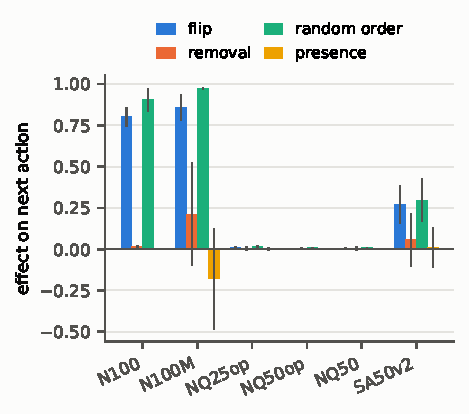
\includegraphics[width=\columnwidth]{figures/fig_dissociation.pdf}
  \caption{Flip, removal, random-order and presence effects at the first decision point by arm (seed means, 95\% $t$ intervals; primary test population).}
  \label{fig:dissociation}
\end{figure}

Table~\ref{tab:seen} repeats the main read-outs on the 280 \texttt{valid\_seen} test games, whose rooms come from training floor plans. The flip, removal and random-order effects are close to those on the primary population in every arm. The exception is the learnable--unlearnable difference in \arm{N100}, which is 0.066 here and 0.008 on the primary population.

At the first decision point, the flip based on the model's own prediction and the flip based on the template ranking for the same foil class differ by $-$0.055 in \arm{N100} (the template is followed slightly more often), $-$0.051 in \arm{N100M}, $-$0.015 in \arm{SA50v2}, and 0.000 in \arm{NQ50op} (this checks an assumption of the imitator reference).

Table~\ref{tab:later} gives the flip effect at later decision points for every arm, and Figure~\ref{fig:dissociation} shows the flip, removal, random-order and presence effects together.
